\chapter{User Manual}
\begin{figure}[H]
	\centering
	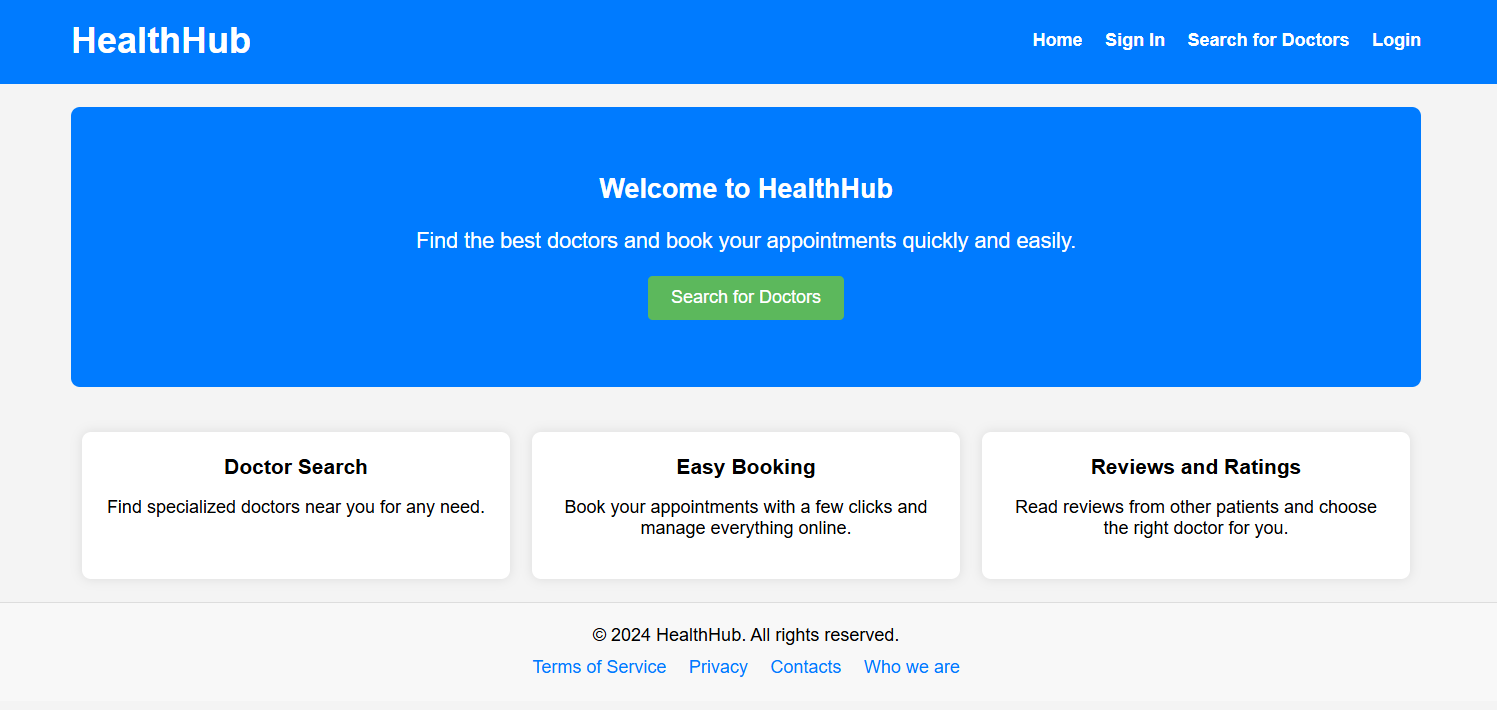
\includegraphics[width=0.8\textwidth]{resources/homepage.png}
	\caption{Home Page of the HealthHub Application}
	\label{fig:homepage}
\end{figure}

\section{Patient}
\subsection{Signup and Login Process}
From the Home Page, users can initiate the authentication process by selecting the \textit{"Sign In"} option located at the top-right corner of the interface.

\begin{figure}[H]
	\centering
	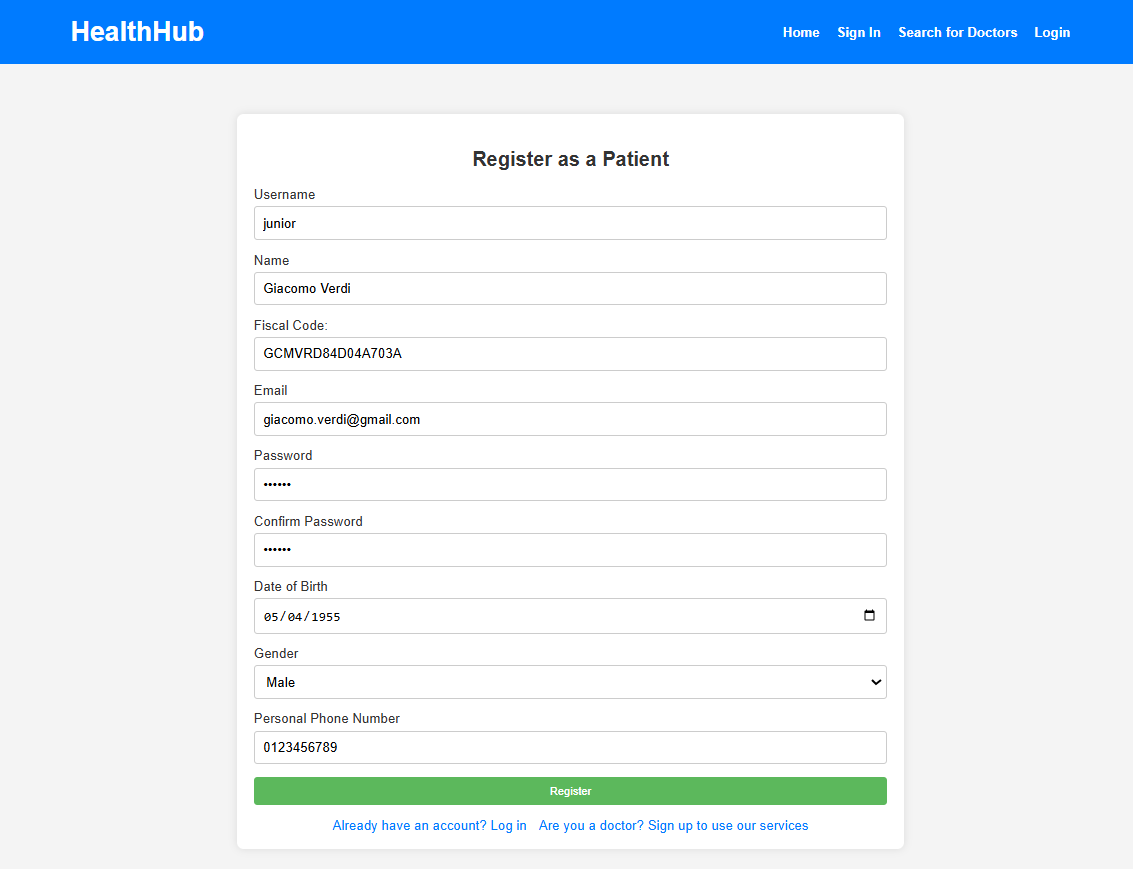
\includegraphics[width=0.8\textwidth]{resources/patient-register.png}
	\caption{Patient Registration Form}
	\label{fig:patient-register}
\end{figure}

Upon accessing the registration interface, a patient may create a new account. Alternatively, users who already possess valid credentials can proceed to the login form.

\begin{figure}[H]
	\centering
	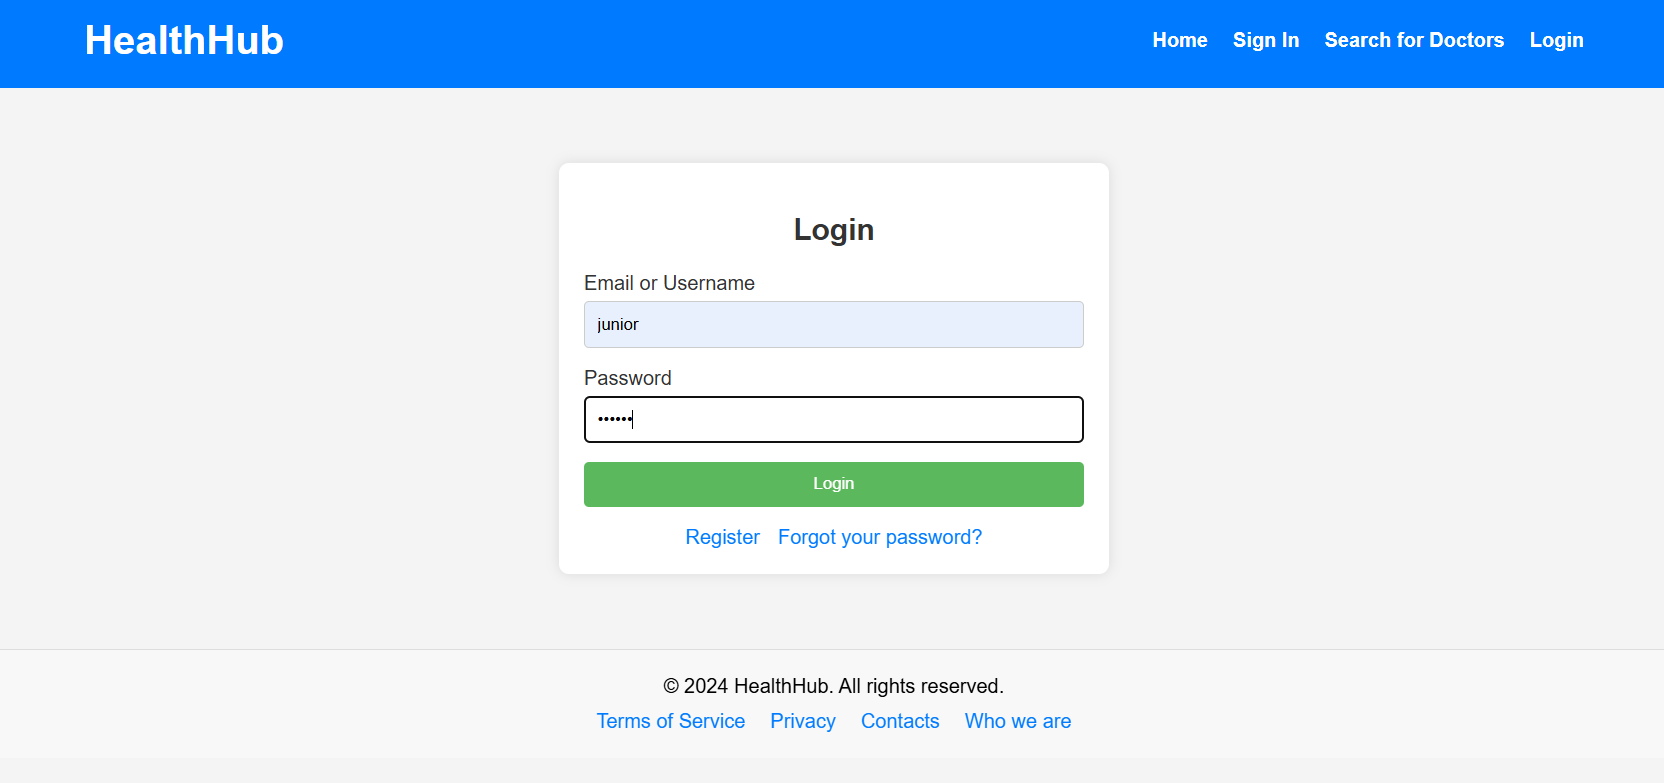
\includegraphics[width=0.8\textwidth]{resources/login-patient.png}
	\caption{Patient Login Form}
	\label{fig:login-patient}
\end{figure}

The login interface also provides auxiliary navigation: by selecting the \textit{Register} button, users are redirected to the registration form. Additionally, by selecting the \textit{Forgot Password} option, users can initiate the password recovery process. This procedure simulates the dispatch of a recovery link to the registered e-mail address.

\begin{figure}[H]
	\centering
	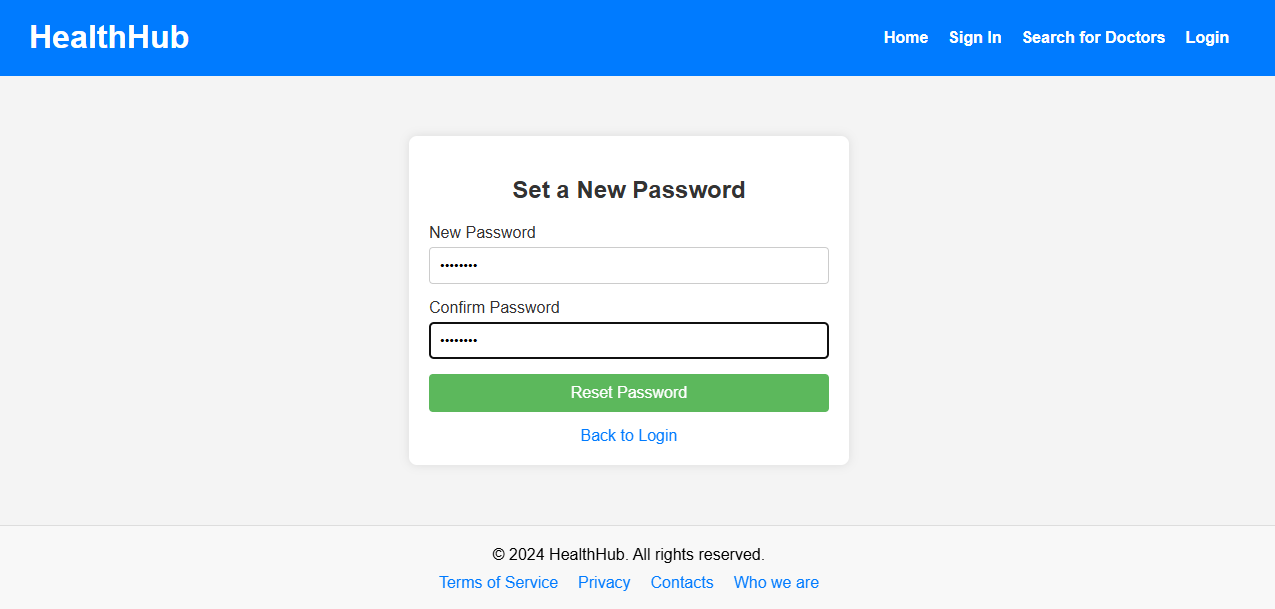
\includegraphics[width=0.6\textwidth]{resources/recover1.png}
	\caption{Password Recovery Request Form}
	\label{fig:recover1}
\end{figure}

\begin{figure}[H]
	\centering
	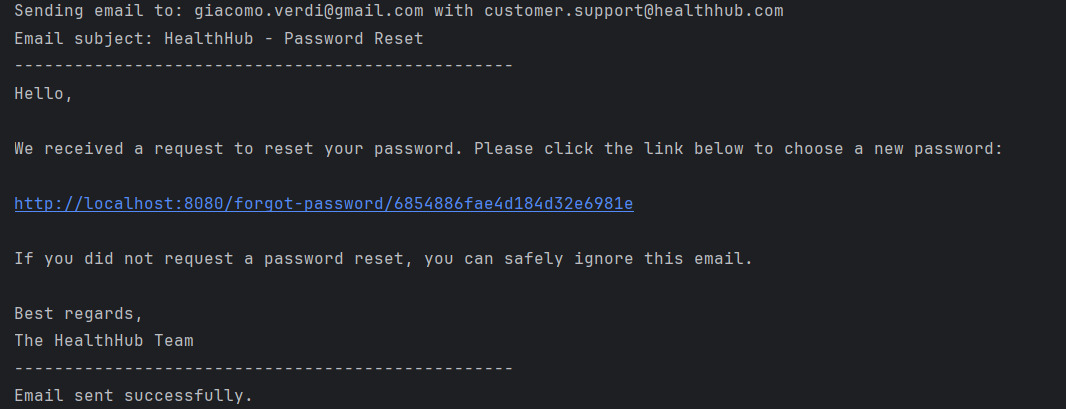
\includegraphics[width=0.6\textwidth]{resources/recover2.png}
	\caption{Confirmation of Email Dispatch}
	\label{fig:recover2}
\end{figure}

\begin{figure}[H]
	\centering
	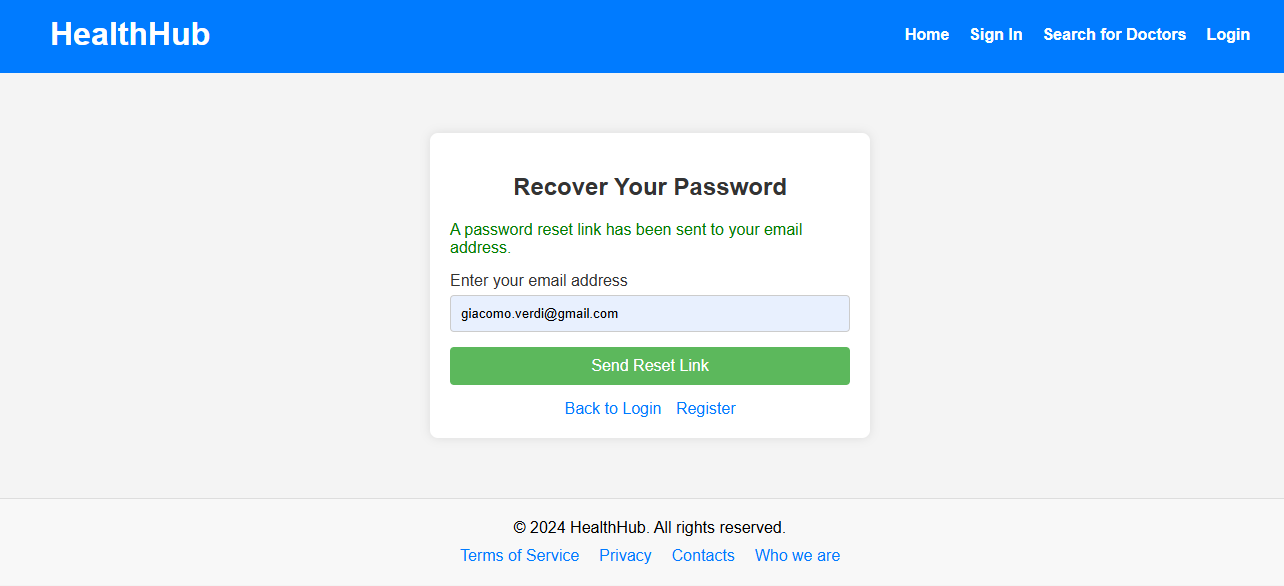
\includegraphics[width=0.6\textwidth]{resources/recover3.png}
	\caption{Password Successfully Updated}
	\label{fig:recover3}
\end{figure}

Once authenticated, the user is redirected to the personalized Patient Home Page. This dashboard provides access to core functionalities including doctor search, profile management, appointment tracking, and the display of favorited doctors—specifically those who have been reviewed or endorsed by the user. A recommendation system enhances this section by suggesting relevant doctors based on the patient's interaction history.

\begin{figure}[H]
	\centering
	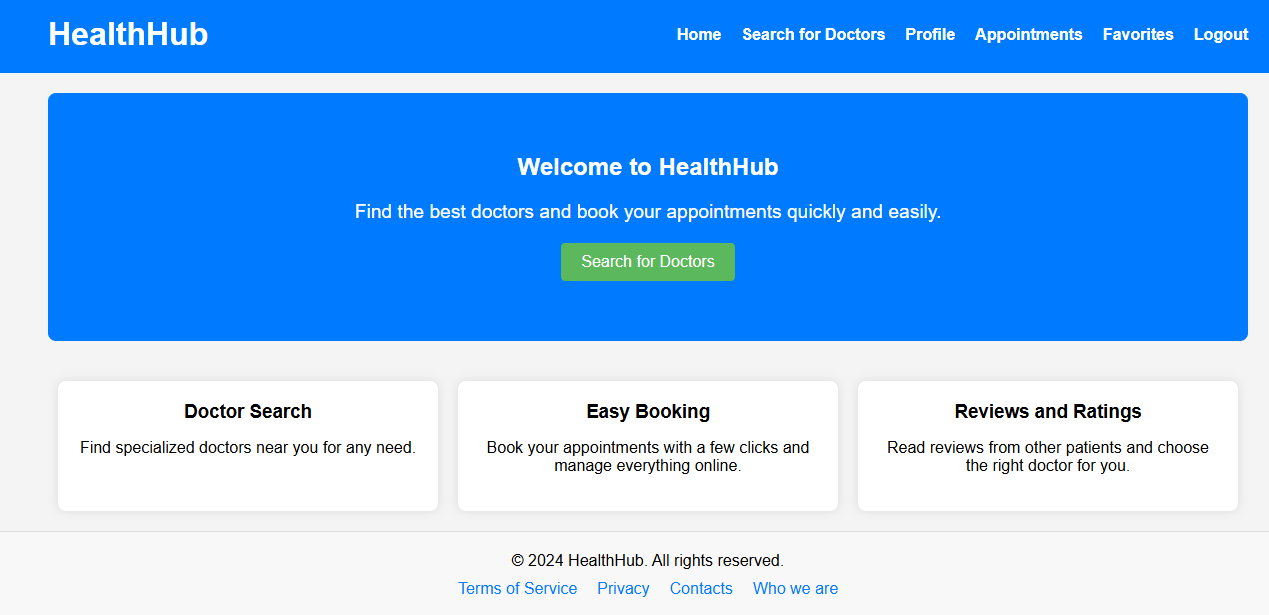
\includegraphics[width=0.8\textwidth]{resources/logged-patient.png}
	\caption{Patient Dashboard After Login}
	\label{fig:logged-patient}
\end{figure}

\subsection{Doctor Profile and Appointment Booking}
By selecting the \textit{"Search for Doctors"} option, users can enter a query string that may consist of a doctor's name, medical specialization, city, province, or a combination of these criteria.

\begin{figure}[H]
	\centering
	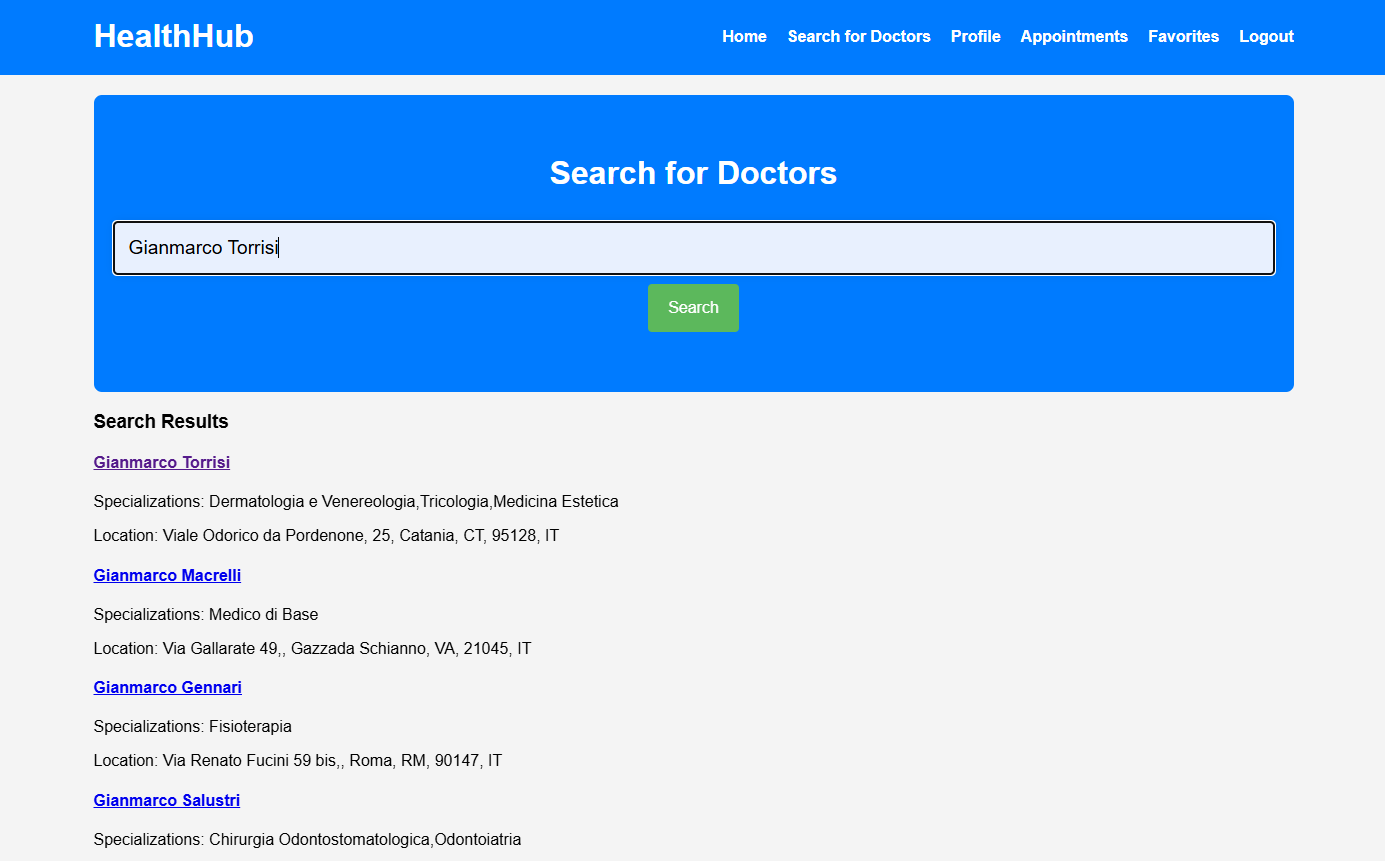
\includegraphics[width=0.8\textwidth]{resources/search-doctor.png}
	\caption{Doctor Search Interface}
	\label{fig:search-doctor}
\end{figure}

After performing a search, the user can select a doctor from the resulting list to access the corresponding public profile page.

The doctor's profile page displays information regarding the available types of visits and the corresponding fees. From this page, the user can book an appointment by selecting a specific visit type. An optional note can be attached to the appointment request to communicate additional information to the doctor.

\begin{figure}[H]
	\centering
	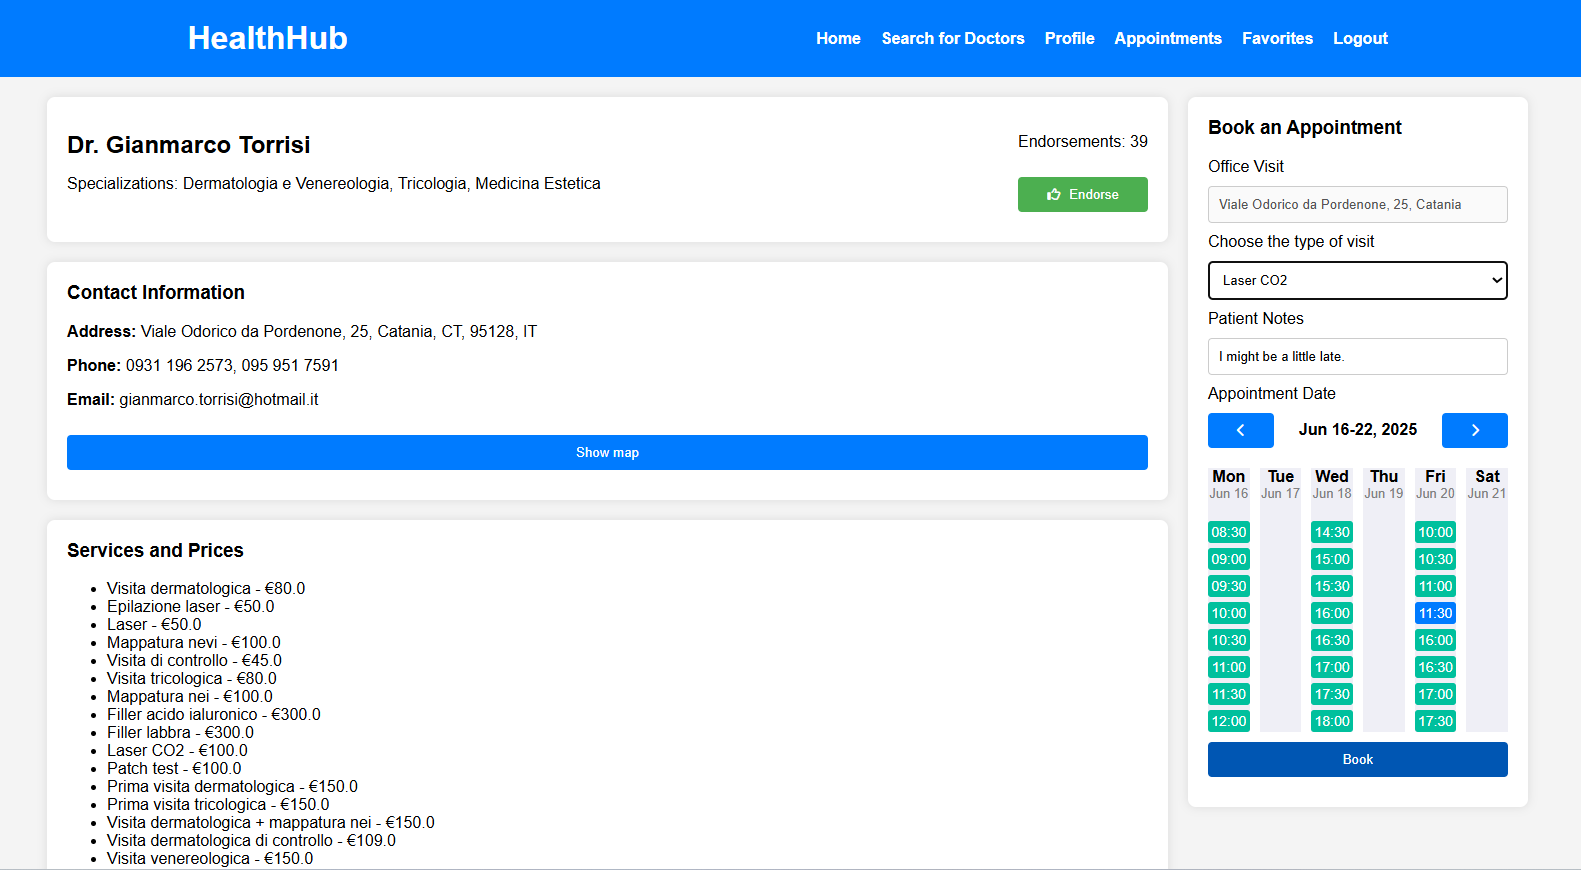
\includegraphics[width=0.8\textwidth]{resources/book-appointment.png}
	\caption{Appointment Booking Interface}
	\label{fig:book-appointment}
\end{figure}

Furthermore, users have the option to endorse the doctor or leave a review. However, reviews are only permitted if the patient has attended at least one appointment with the doctor in question. This ensures the authenticity and reliability of the feedback provided.

\begin{figure}[H]
	\centering
	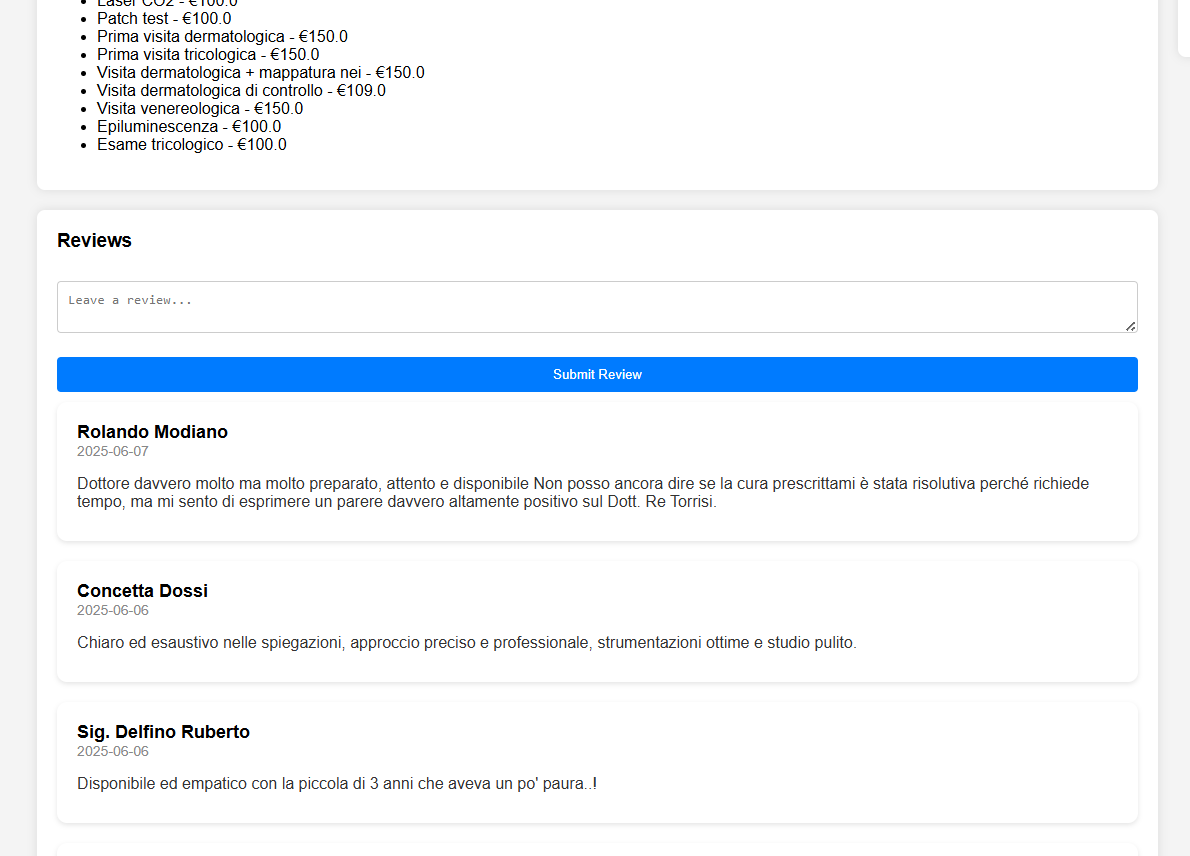
\includegraphics[width=0.8\textwidth]{resources/review-doctor.png}
	\caption{Doctor Review Interface (Note: Reviewing is allowed only after completing at least one appointment with the doctor)}
	\label{fig:review-doctor}
\end{figure}

\section{Doctor}

\subsection{Overview}
Doctors have access to a dedicated interface that allows them to manage their appointments, review patient feedback, and edit their personal and professional information. They can also monitor key analytics related to their activity and configure their weekly availability through calendar templates.

\subsection{Dashboard}

\begin{figure}[!h]
	\centering
	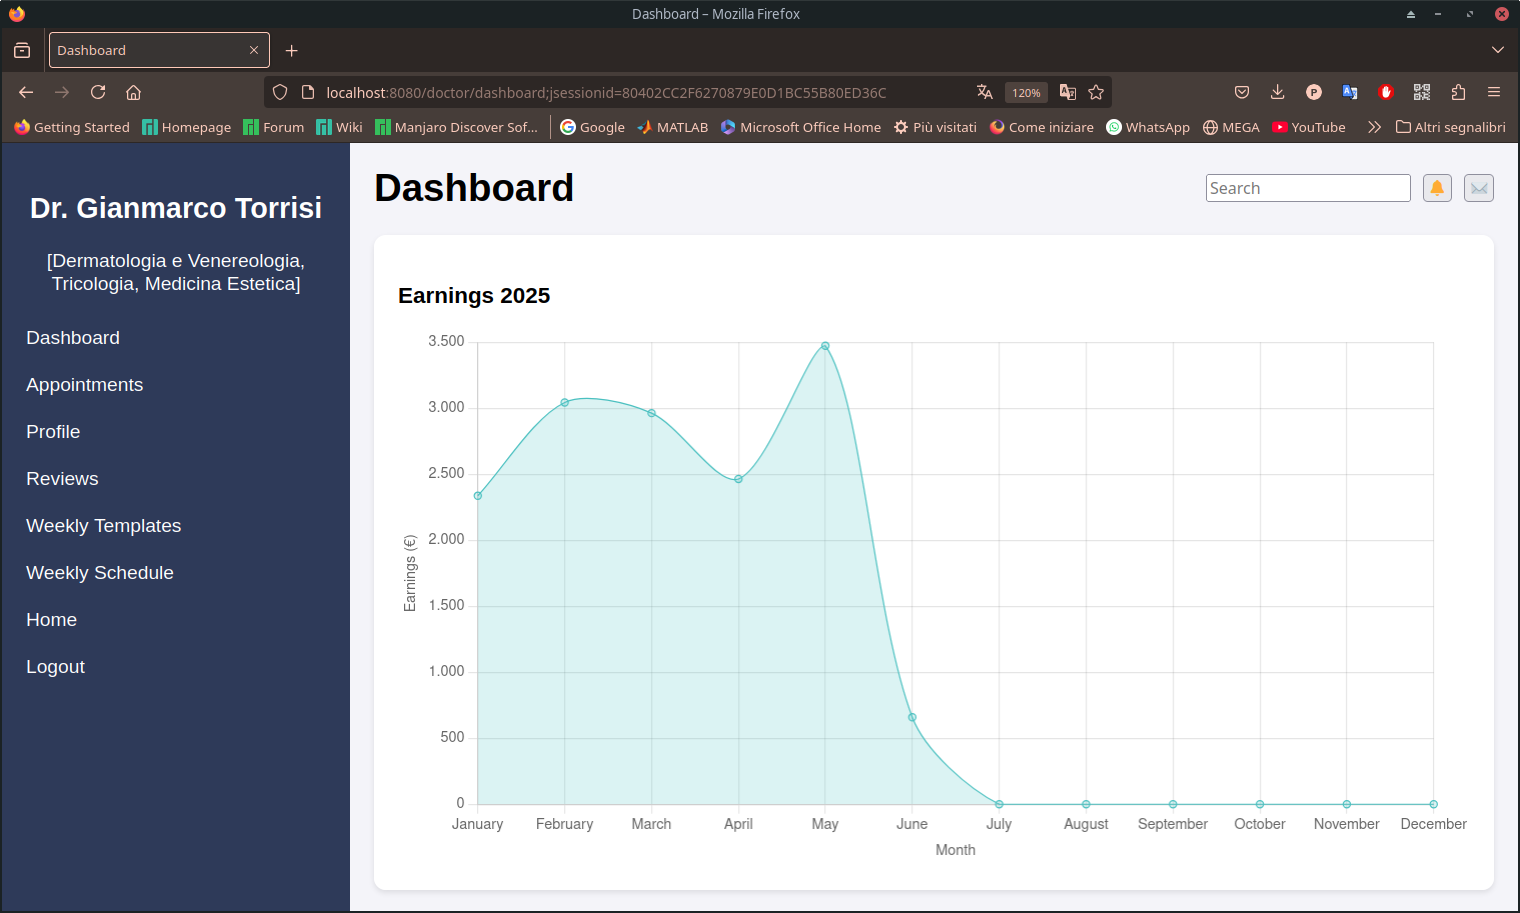
\includegraphics[scale=0.30]{resources/screenshots/doctor_ui/earnings_linechart.png}
	\caption{Line chart displaying earnings by month for the current year.}
	\label{fig:earnings_linechart}
\end{figure}

\begin{figure}[!h]
	\centering
	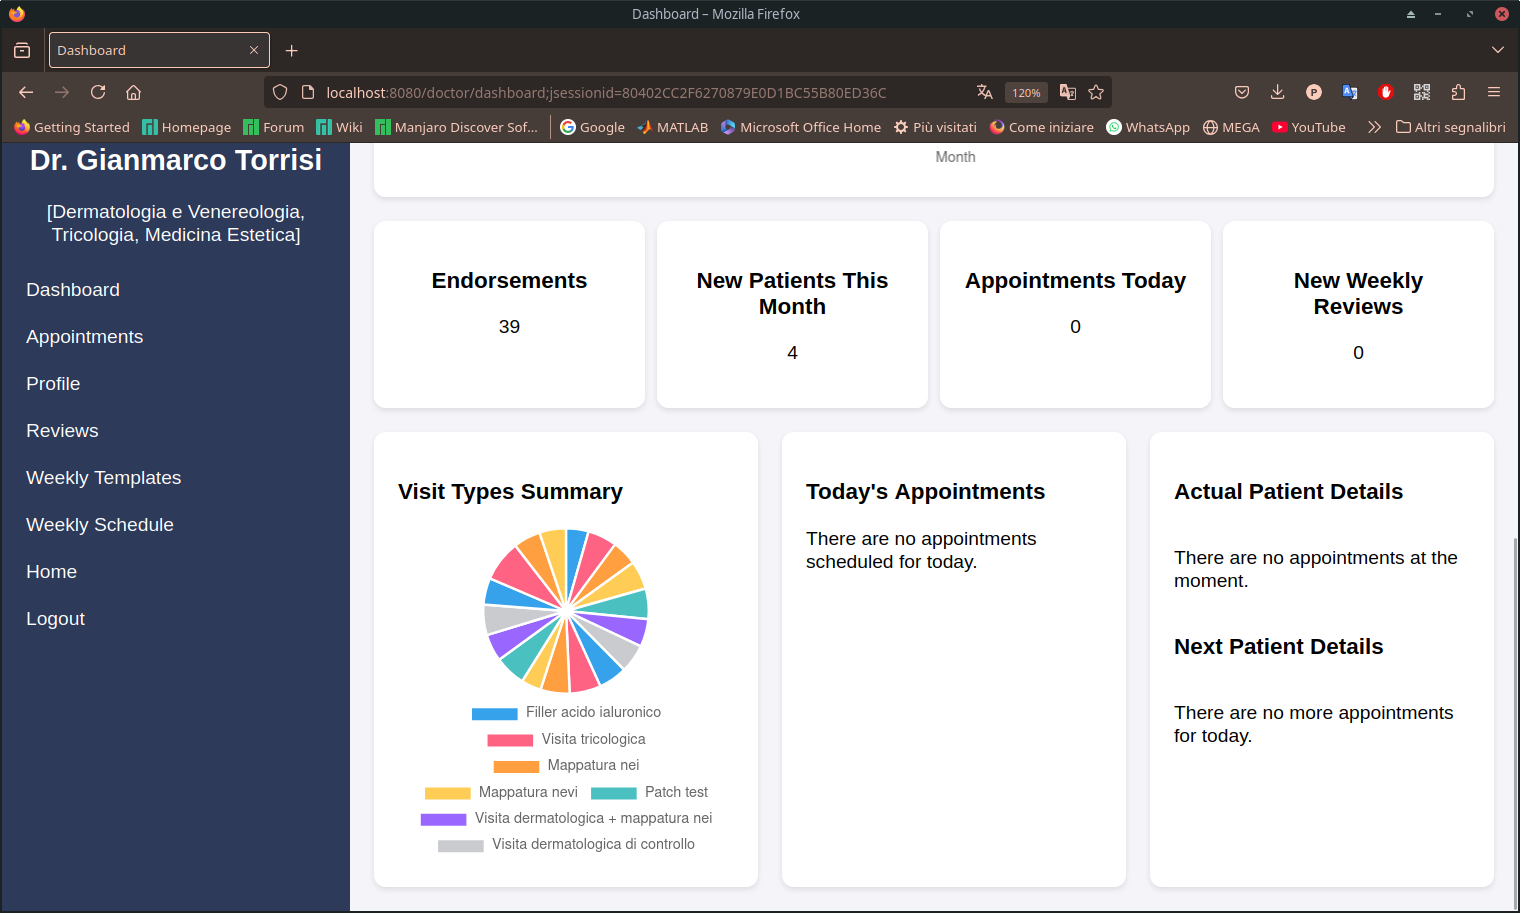
\includegraphics[scale=0.30]{resources/screenshots/doctor_ui/dashboard_bottom.png}
	\caption{Pie chart showing the distribution of services provided by the doctor.}
	\label{fig:services_piechart}
\end{figure}

The dashboard provides doctors with an overview of their current performance. It includes:
\begin{itemize}
	\item A line chart displaying total earnings for the current year.
	\item A pie chart illustrating the distribution of services provided.
	\item A summary of today's appointments, with access to detailed information.
	\item A preview of the next scheduled patient.
	\item Key performance indicators, including:
	\begin{itemize}
		\item \textbf{Endorsements}
		\item \textbf{New Patients This Month}
		\item \textbf{Appointments Today}
		\item \textbf{New Weekly Reviews}
	\end{itemize}
\end{itemize}

\subsection{Appointment List}
This section allows the doctor to view a comprehensive list of appointments. The list can be filtered by date, and each entry provides access to detailed information or cancellation options.

\begin{figure}[!h]
	\centering
	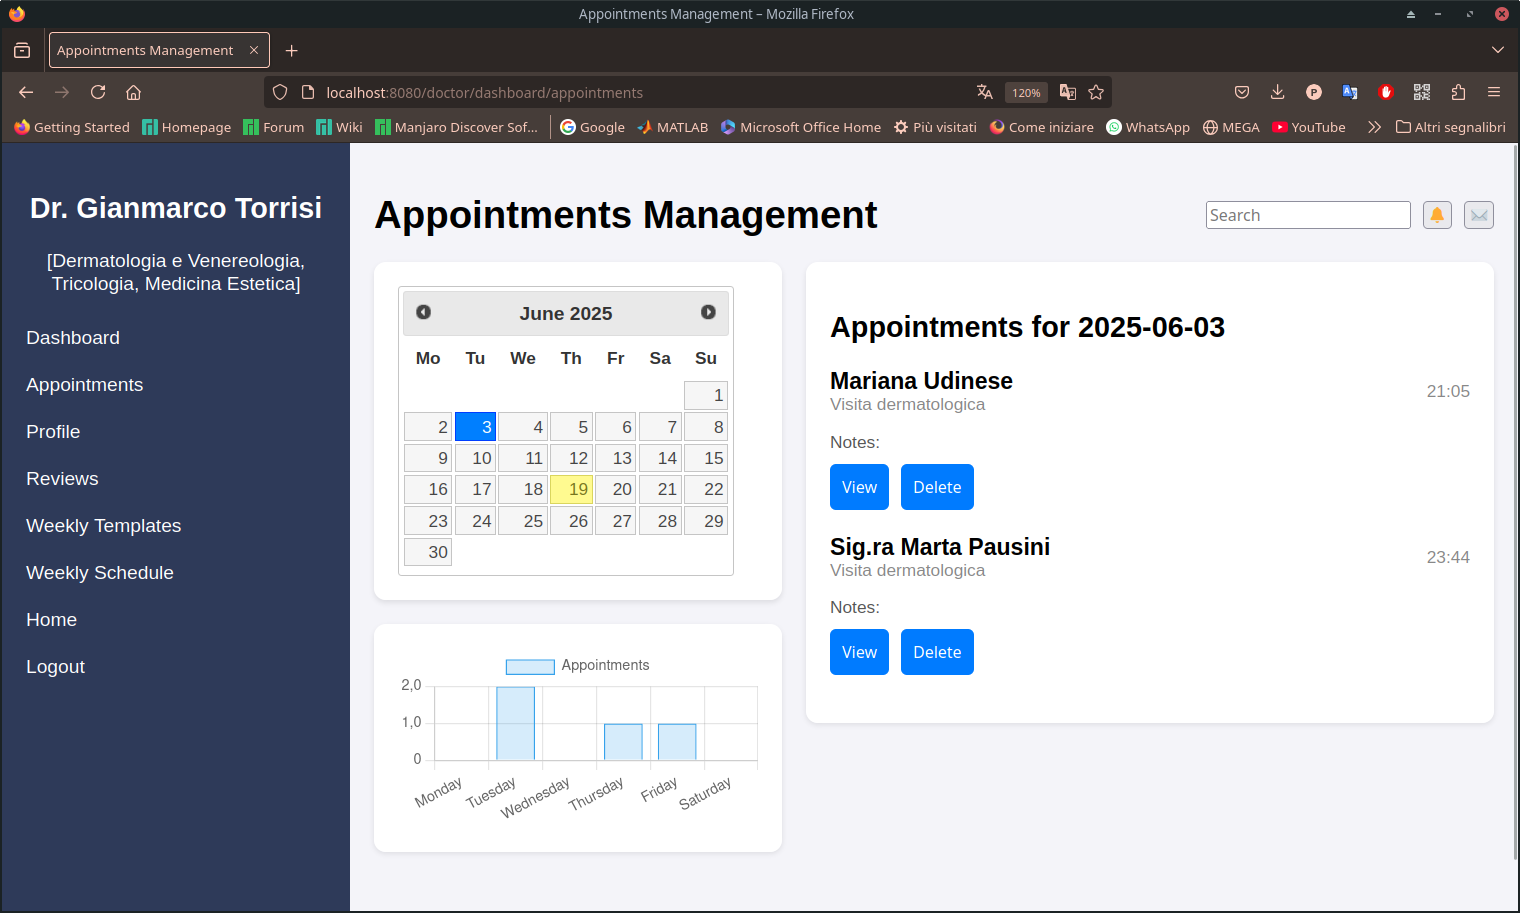
\includegraphics[scale=0.30]{resources/screenshots/doctor_ui/appointments.png}
	\caption{Appointment list with filtering options.}
	\label{fig:appointment_list}
\end{figure}

\subsection{Personal Profile}

\begin{figure}[!h]
	\centering
	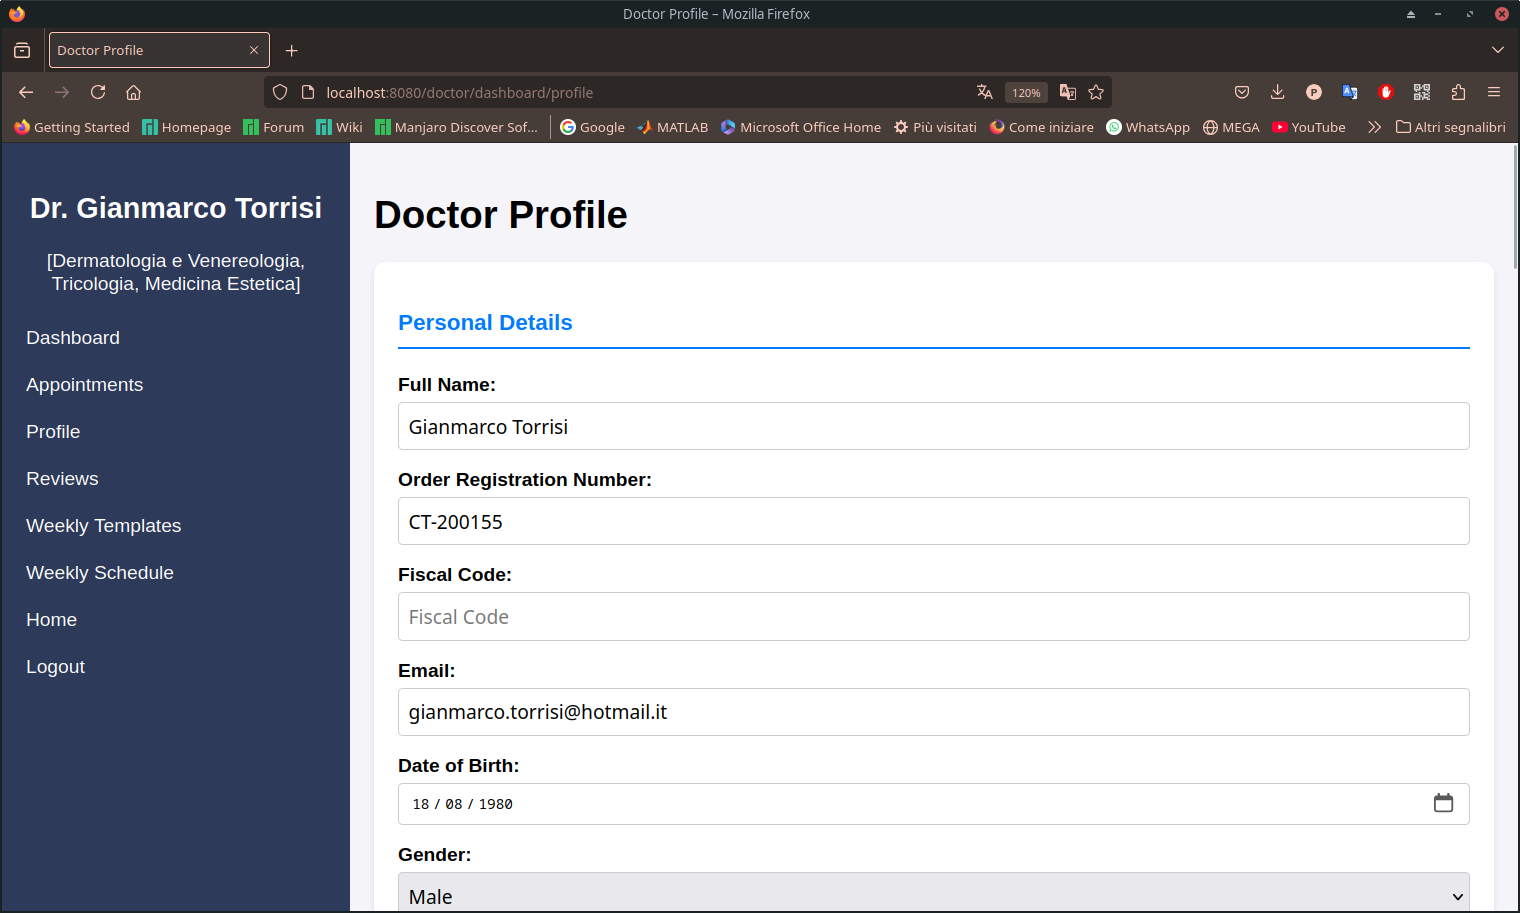
\includegraphics[scale=0.30]{resources/screenshots/doctor_ui/personal_info.png}
	\caption{Doctor's profile page with editable fields.}
	\label{fig:doctor_profile}
\end{figure}

\begin{figure}[!h]
	\centering
	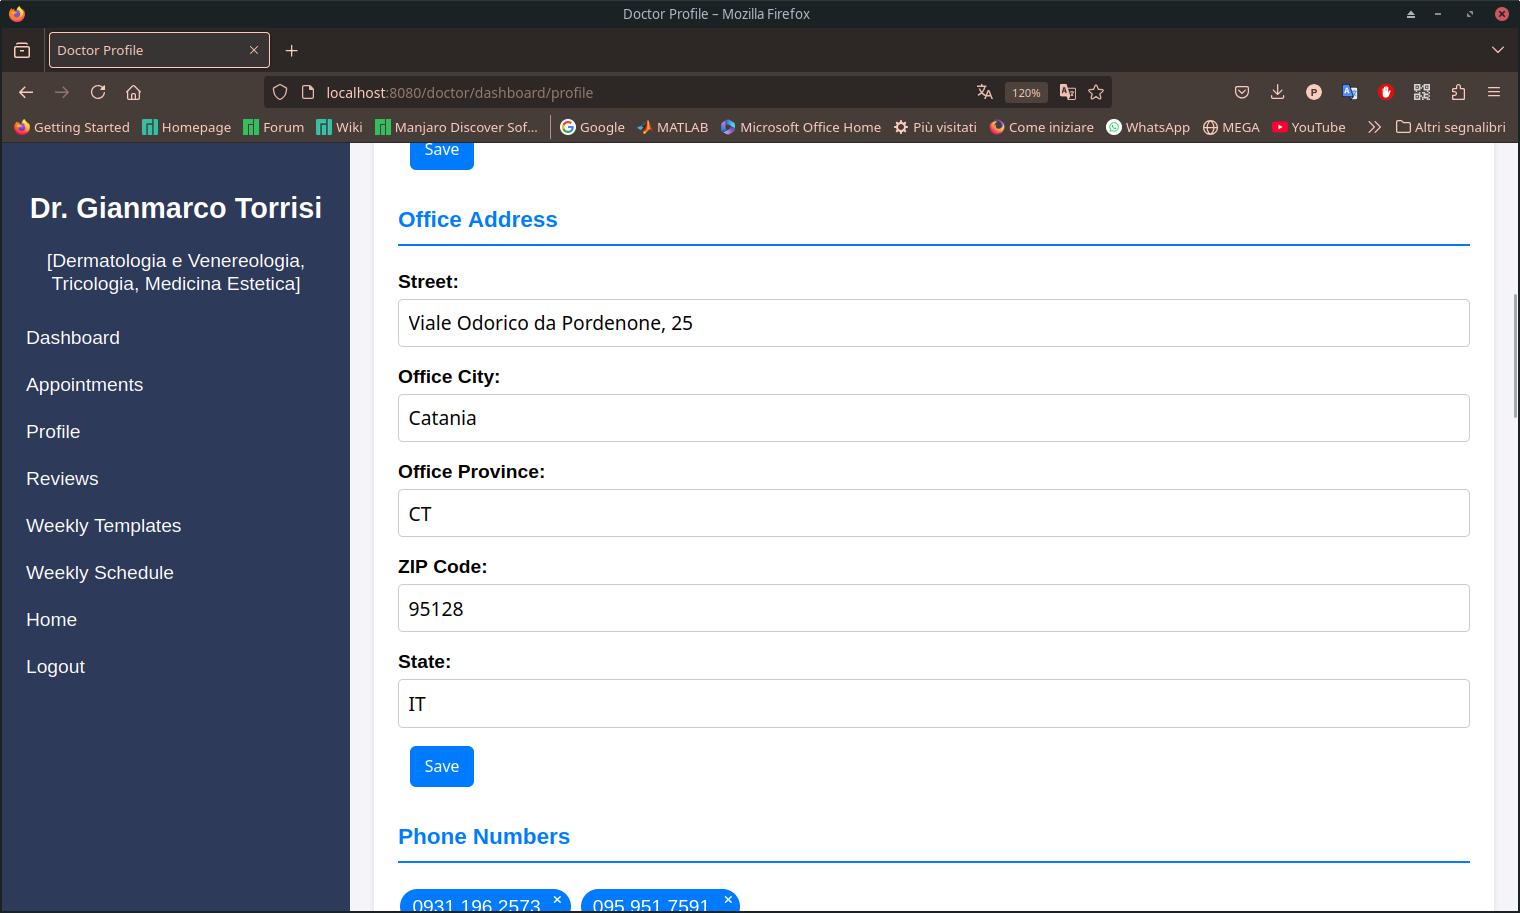
\includegraphics[scale=0.30]{resources/screenshots/doctor_ui/address.png}
	\caption{Doctor's office address and contact information.}
	\label{fig:doctor_address}
\end{figure}

\begin{figure}[!h]
	\centering
	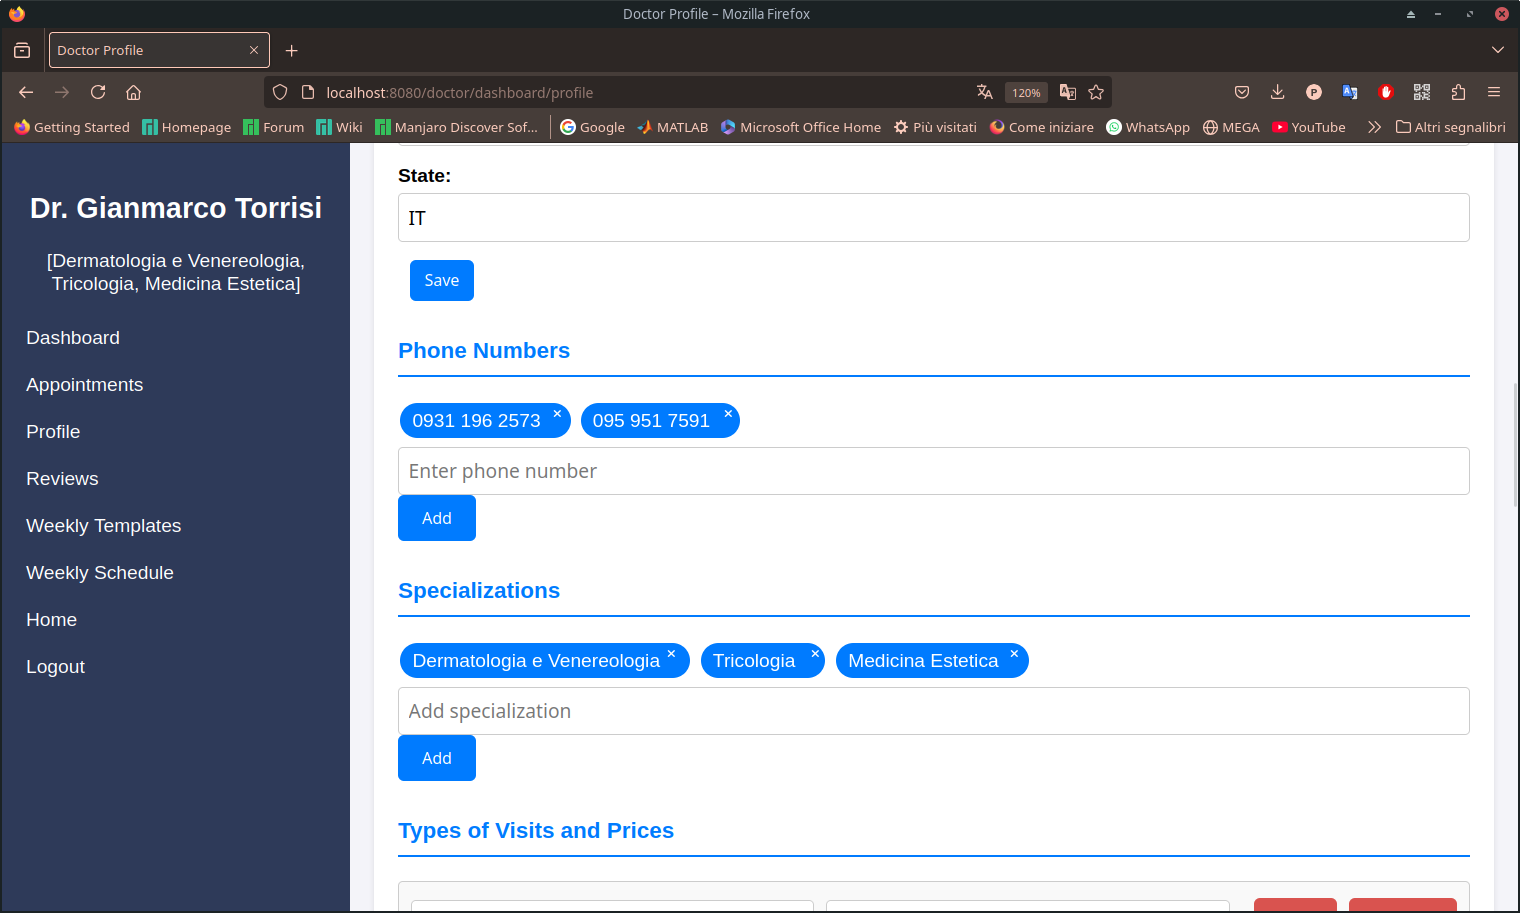
\includegraphics[scale=0.30]{resources/screenshots/doctor_ui/specializations.png}
	\caption{Medical specialties that the doctor can add or edit.}
	\label{fig:doctor_specialties}
\end{figure}

\begin{figure}[!h]
	\centering
	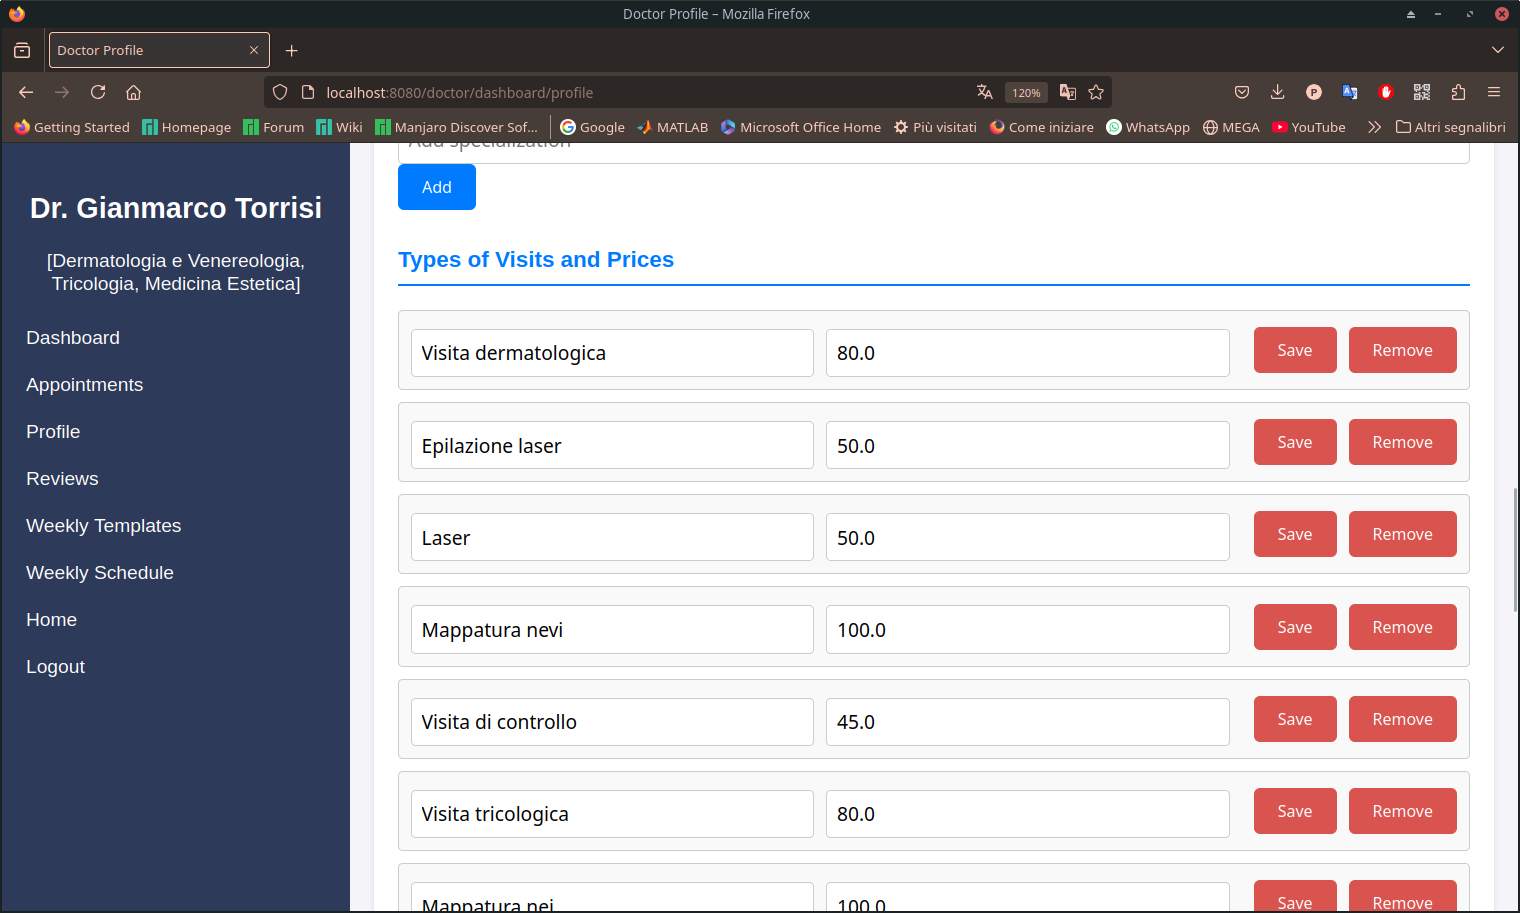
\includegraphics[scale=0.30]{resources/screenshots/doctor_ui/services.png}
	\caption{Services offered by the doctor, including name and cost.}
	\label{fig:doctor_services}
\end{figure}

In the profile section, doctors can view and edit their personal details and professional information. Specifically, they can:
\begin{itemize}
	\item Update their office address, phone numbers, and email address.
	\item Provide a list of services they offer, including the name and cost of each.
	\item Add or edit their medical specialties.
	\item Change their account password.
\end{itemize}

\subsection{Review Page}

\begin{figure}[!h]
	\centering
	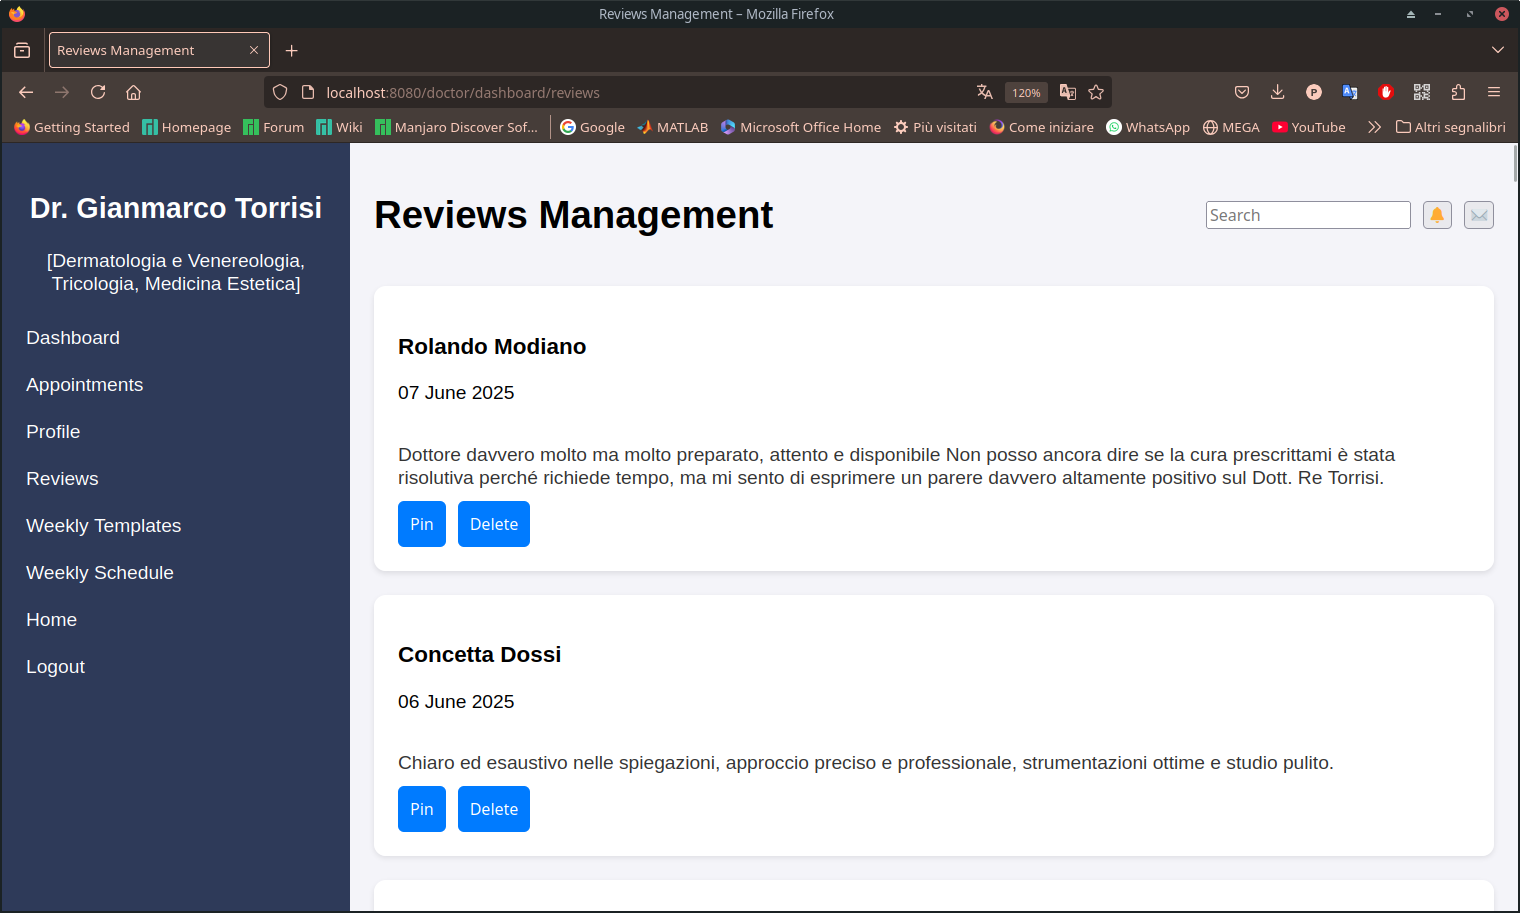
\includegraphics[scale=0.30]{resources/screenshots/doctor_ui/reviews.png}
	\caption{Patient reviews with options to delete or view details.}
	\label{fig:patient_reviews}
\end{figure}

Doctors can browse the reviews left by their patients. If necessary, inappropriate or outdated reviews can be deleted directly from this section.

\subsection{Calendar Templates}

\begin{figure}
	\centering
	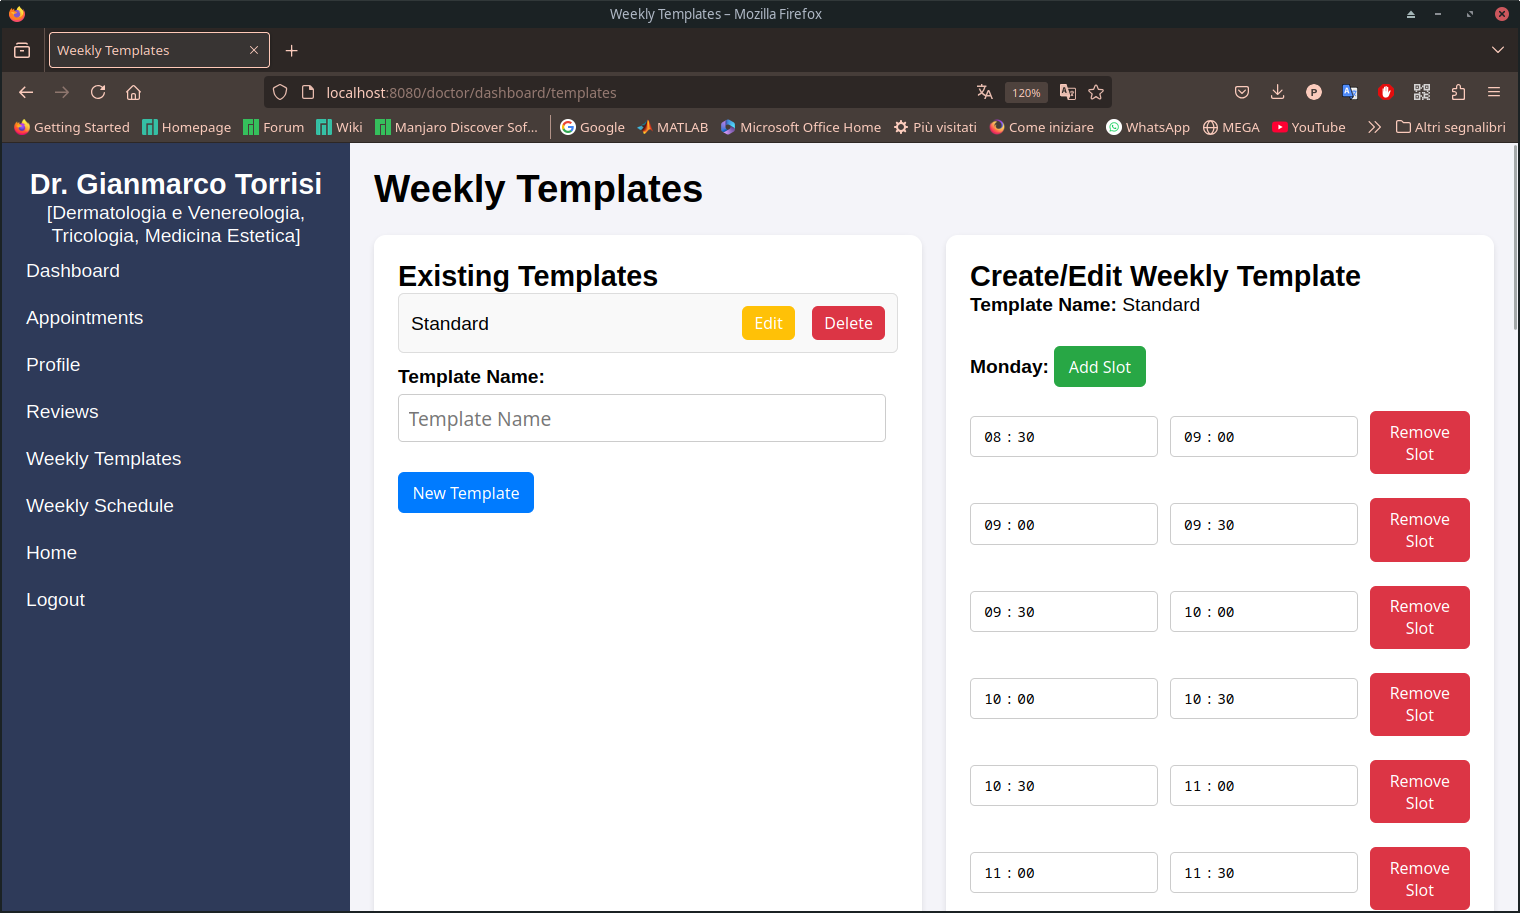
\includegraphics[scale=0.30]{resources/screenshots/doctor_ui/template.png}
	\caption{Calendar templates for managing weekly availability.}
	\label{fig:calendar_templates}
\end{figure}

In this area, doctors can create and manage calendar templates that define their weekly availability. Each template includes:
\begin{itemize}
	\item A custom name for the template.
	\item For each day of the week, a list of time slots indicating availability.
\end{itemize}
Templates can be edited or deleted at any time.

\subsection{Weekly Schedule}

\begin{figure}[!h]
	\centering
	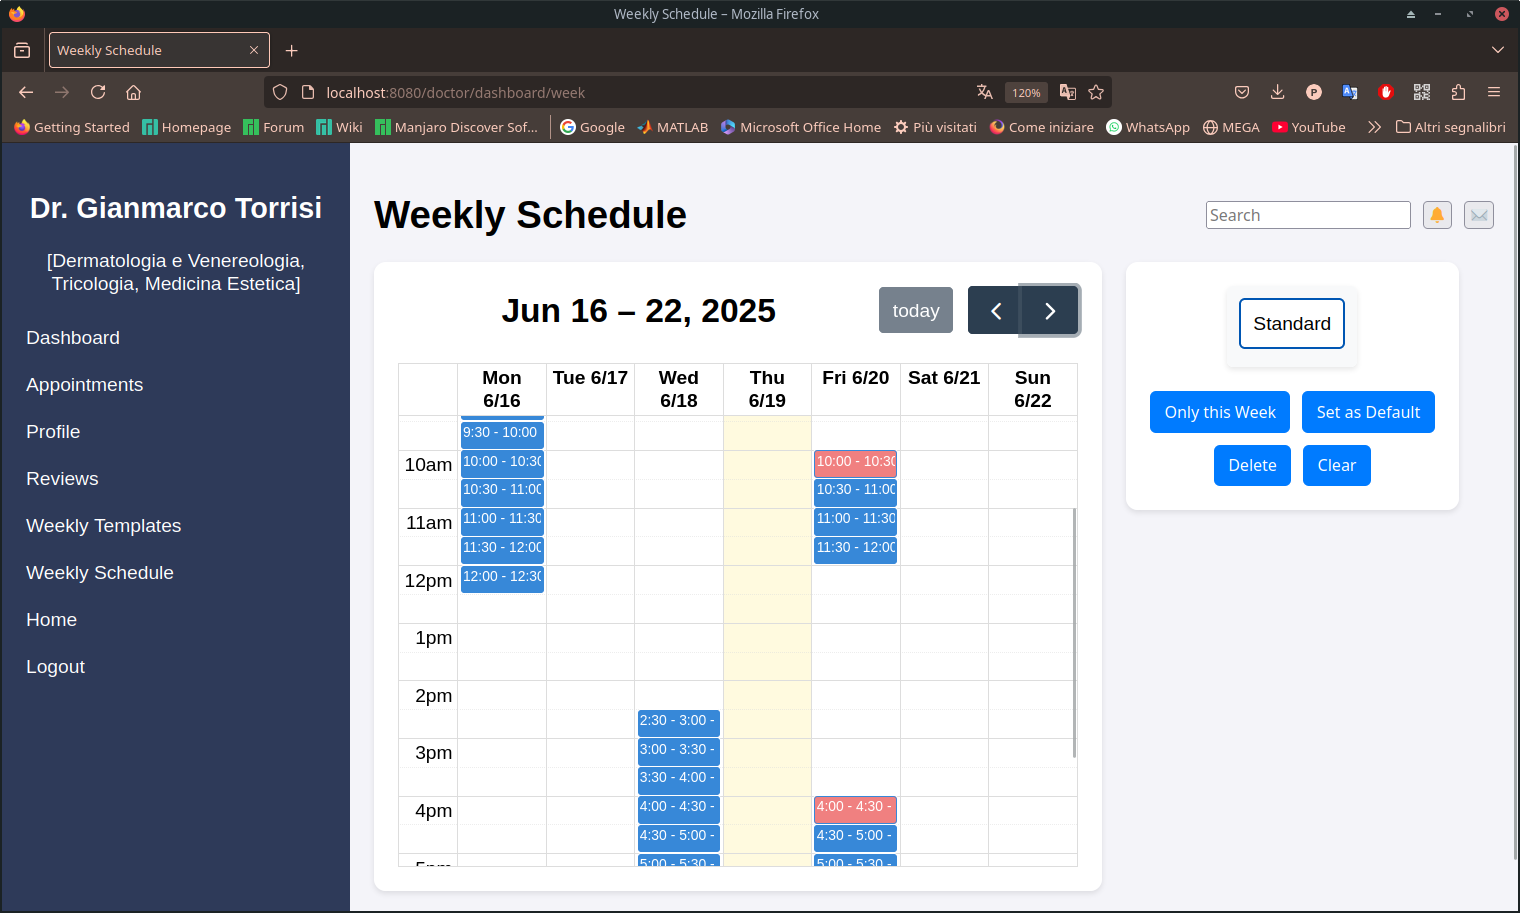
\includegraphics[scale=0.30]{resources/screenshots/doctor_ui/schedule.png}
	\caption{Weekly schedule with booked and available time slots.}
	\label{fig:weekly_schedule}
\end{figure}

The schedule page allows doctors to view and manage their weekly appointment calendar. Key features include:
\begin{itemize}
	\item Viewing existing appointments.
	\item Assigning a predefined calendar template to a specific week.
	\item Deleting the calendar for a selected week.
\end{itemize}

The calendar visually distinguishes between booked slots (highlighted in red) and available time slots (in blue), allowing for quick assessment and management.